\chapter{Research problems on social media}
\label{chap:direction}
In recent years, the research on social network in data mining area
is becoming more and more popular. Generally, the researchers are
interested in the following problems which are related to the
information diffusion: 1) influence maximization;
2) community Detection; 3) link prediction. In this chapter, we will
survey state-of-the-art work of the research on this three problems.

\section{Influence maximization}

The influence maximization problem is to find a group of nodes, which
we can call them influential nodes, as the seeds to maximize the
influence. 

Kempe et al.~\cite{kempe2003maximizing} studied the influence
maximization problem using two basic models, namely, the
independent cascade model and linear threshold mode. They proved that
this maximization problem under both the linear threshold model and
independent cascade model is NP-hard and proposed a greedy
alogrithm. The data they used is a collaboration graph which is
obtained from the co-authorship in physics publications. From the
experiment, they showed that the greedy algorithm significantly
outperformed the high-degree and centrality heuristics, which is
consistent with the conclusion drawn in the sociology literature. Also,
they mathematically proved that the greedy algorithm is a
$(1-e^{-1})$-approximation algorithm by using an analysis framework
based on submodular functions.

Based on the submodularity property of the maximization problem,
Leskovec et al. proposed a new greedy
algorithm called CELF, which is short for ``Cost-Effective Lazy Forward''~\cite{leskovec2007cost},
guaranteeing at least a constant fraction of the optimal
solution. In addition, they claimed that CELF could be as 700 times
fast as the simple greedy algorithm. They used this algorithm for the Battle of Water Sensor Network (BWSN), which is to
find the best sensor placements for a water distribution network in a real metropolitan area. Also, they did the experiment on blog data
to show the performance of the algorithm.

Chen et al. in their work~\cite{chen2009efficient} further improved
the greedy algorithm and called the new algorithm MixedGreedy and NewGreedy. The data they
used is the same as ~\cite{kempe2003maximizing}. The improvement
of the NewGreedy is to remove the edges that won't contribute to the
diffusion any more. MixedGreedy combines the CELF and NewGreedy
together: at the first round, the NewGreedy is applied and for the
rest, the CELF is applied. Another major contribution of their work is
that they presented a heuristic algorithm called DegreeDiscount which is
significantly faster than the greedy algorithm. However, it cannot
guarantee the constant factor of the optimal result.

Masahiro Kimura et al.~\cite{kimura2010extracting} proposed a method
of efficiently estimating all the marginal influence degrees of a
given set of nodes on the basis of bond percolation and graph theory,
and applied it to approximately solve the influence maximization
problem by the greedy algorithm. They used large-scale real
networks (i.e. blog networks) to demonstrate that the proposed
 method was much more efficient than ~\cite{kempe2003maximizing}.

\section{Community dectection}

The problem of community dectection is how to group the nodes in one social network together based on some particular properties of the nodes or some strategies.

Generally, there are two structures of the community: the overlapping community structure and the non-overlapping community structure. The overlapping community structure means for every node in the graph, i can belong to more than one communities and the non-overlapping community structure means for every node it can belong only one communities. 

Blondel et al. have analyzed a network of mobile phone communications between users of a Belgian phone operator~\cite{blondel2008fast}.
The vertices of the graph are 2.6 millions and the edges are weighted by the cumulative duration of phone calls between users in the observation time frame. The clustering analysis, performed with a fast hierarchical modularity optimization technique
developed by the authors, delivers six hierarchical levels. The highest level consists of 261 groups
with more than 100 vertices, which are clearly arranged in two main groups, linguistically homogeneous, reflecting the
linguistic split of Belgian population. 

Tyler et al.\cite{tyler2005mail} studied a network of e-mail exchanges between people
working at the HP Labs. They applied the same modified version of the Girvan-Newman algorithm that two of the authors have used
to find communities of related genes~\cite{wilkinson2004method}. The method enables one to measure the degree of membership
of each vertex in a community and allows for overlaps between communities. The detected clusters matched quite closely
the organization of the Labs in departments and project groups, as
confirmed by interviews conducted with researchers.

\begin{figure}[!htb]
  \centering
  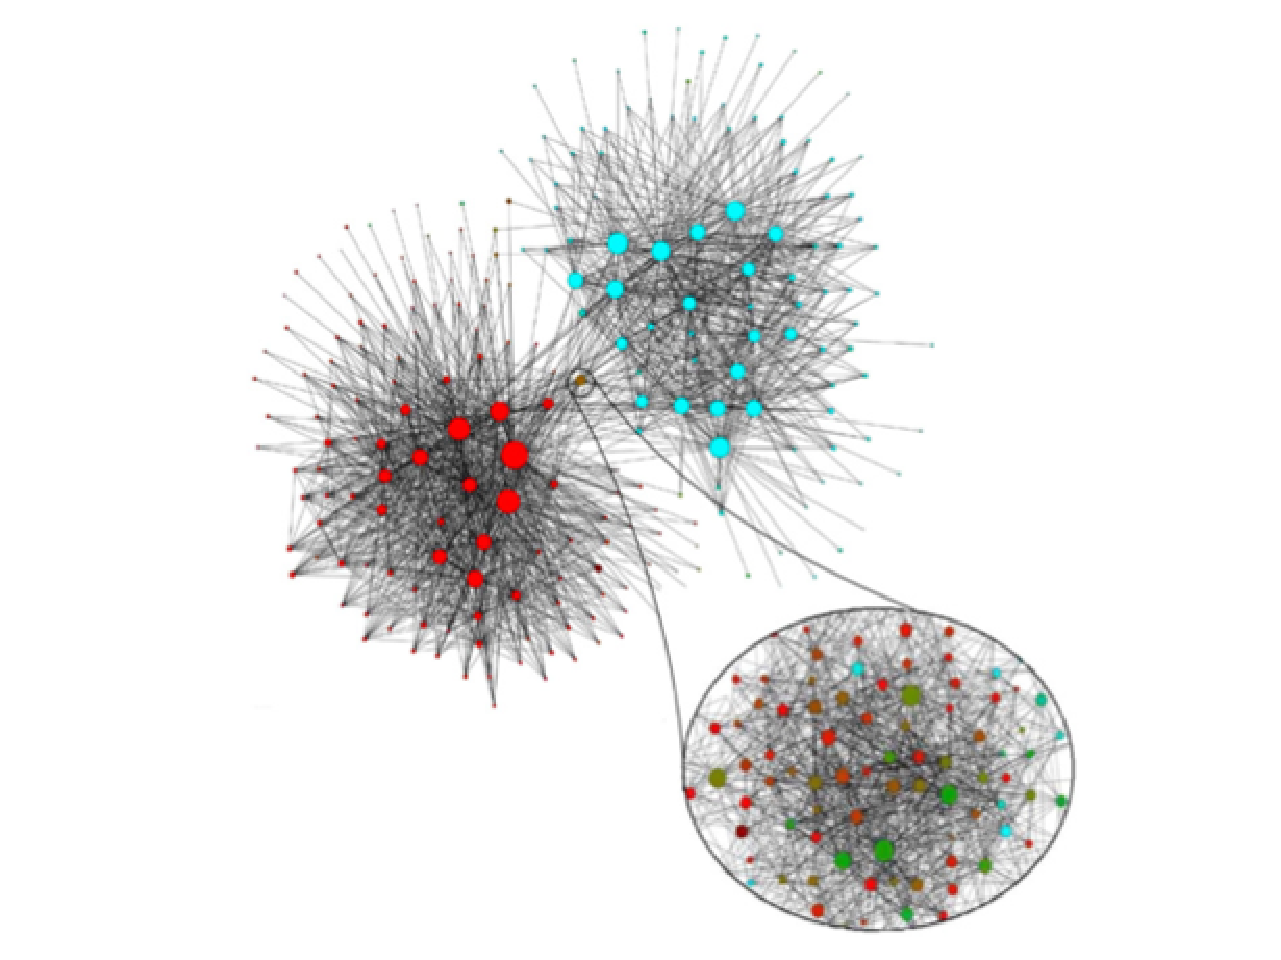
\includegraphics[width = 340]{figures/community.eps}
  \caption{Community structure of a social network of mobile phone
    communication in Belgium. Dots indicate subcommunities at the
    lower hierarchical level (with more than 100 people) and are
    colored in a red–green scale to represent the level of
    representation of the two main languages spoken in Belgium (red
    for French and green for Dutch). Communities of the two larger
    groups are linguistically homogeneous, with more than 85\% of
    people speaking the same language. Only one community (zoomed),
    which lies at the border between the two main aggregations, has a
    more balanced distribution of languages.~\cite{blondel2008fast}}
  \label{fig:community}
\end{figure}


Traud et al.~\cite{traud2008community} used
anonymous Facebook data to create networks of friendships between students of different American universities, where
vertices/students are connected if they are friends on Facebook. Communities were detected by applying a variant of
Newman's spectral optimization of modularity: the results were further
refined through additional steps. One of the goals of the study was to
infer relationships between the online and offline lives
of the students. By using demographic information on the students' populations, one finds that communities are organized
by class year or by House (dormitory) affiliation, depending on the university. 

Yuta et al.~\cite{yuta2007gap} observed a gap in the
community size distribution of a friendship network extracted from mixi (mixi.jp), the largest SNS in Japan (as of December 2006). Communities were identified with the fast greedy modularity optimization by~\cite{clauset2004finding}.
Yuta et al. introduced a model where people form new friendships both by ``closing'' ties with people who are friends of friends, and by setting new links with individuals having similar interests. In this way most groups turn out to be either small or large, and medium size groups are rare.

\section{Link prediction}

For some social networks, while it is often possible to directly
observe when nodes become infected, observing individual transmissions
may be very difficult. The reason is that people cannot only get the
information from the social network, but also get it from offline
activity (e.g. a conversation) or other media. Also, we want to predict
which nodes will be infected in the future. We call those two problems
together as the link prediction problem. 

Liben-Nowell and Kleinberg proposed one of the earliest link
prediction models that works explicitly on a social network~\cite{liben2003link}. Every
vertex in the graph represents a person and an edge between two
vertices represents the interaction between people. They
concentrated mostly on the performance of various graph-based
similarity metrics for the link prediction task. Hasan et al. extended
this work in two ways~\cite{al2005link}: 1) using the external data
outside of the scope of the graph topology; 2) using various
similarity metrics as the features in a supervised learning setup. 

The link prediction problem has also been studied previously in the context
of relational data and also in the Internet domain, where explicit graph representations were not used. The prediction system proposed in
these works can accept any relational dataset, where the objects in the dataset
are related to each other in any complex manners and the task of the system is
to predict the existence and the type of links between a pair of objects in the
dataset. Probabilistic relational models, graphical model, stochastic relational models, and different variants of these are the main
modeling paradigm used in these works. The advantages of these approaches
include the genericity and ease with which they can incorporate the attributes
of the entities in the model. The disadvantage is that they are usually complex, and
have too many parameters, many of which may not be that intuitive to the user.

The research on social network evolution closely resembles the
link prediction problem. An evolution model predicts the future edges of a network, taking into account some well known attributes of social networks, such
as the power law degree distribution and the small world phenomenon.
This remains the main difference between evolution models and the link prediction models. The former concentrate on the global properties of the network
and the latter model the local states of the network to predict the probability of
the existence of a link between a special pair of nodes in the network. Nevertheless, the ideas from these models have been instrumental for some research
works that directly addressed the task of link prediction.

One of the main challenges of link prediction concerns the evolution of Internet scale social networks like Facebook, MySpace, Flickr, and so on. These
networks are huge in size and highly dynamic in nature for which earlier algorithms may not scale and adapt well. More direct approaches are required to
address these limitations. For instance, Tylenda et. al. shows that utilizing
the time stamps of past interactions, which explicitly utilize the lineage of interactions, can significantly improve the link prediction performance~\cite{tylenda2009towards}. Recently,
Song et. al. used matrix factorization to estimate similarity between the
nodes in a real life social network having approximately 2 millions nodes and
90 millions edges~\cite{song2009scalable}. Any traditional algorithm that aims to compute pair-wise
similarities between vertices of such a big graph is doomed to fail. Recently,
the matrix based factorization works have been extended to the more richer
higher-order models such as tensors.
